\cleardoublepage
\chapter{实验结果与分析}
在本章中,本文将对TimeChain系统进行全面的实验评估,从存储延迟和查询延迟两个关键维度来验证TimeChain设计的有效性。
本文将分析TimeChain在不同查询负载和存储网络条件下的性能表现,并针对系统中的自适应聚合机制、基于共识的节点选择机制和基于LSH树的验证机制进行消融实验,以展示这些技术点对系统性能的具体提升。
通过这些实验,本文旨在展示TimeChain相比于现有解决方案在区块链存储系统中的性能优势。

\section{实验设置}
本文基于一些开源项目(如Hyperledger Fabric和IPFS)实现TimeChain。
本文使用阿里云的50台虚拟机构建了一个基于Hyperledger Fabric的底层区块链系统,每个节点配备2核CPU和4GB内存。
块大小设置为1500个交易,块间隔为1秒。

本文基于一个真实世界的存储网络~\cite{corneo2021surrounded},模拟了分布在世界各地的320个云服务器节点,并基于该集群进行了实验。
每个存储节点配置2核CPU和4GB内存,每个存储节点的存储空间为512GB。
存储节点和网关之间的距离从800公里到6000公里不等,平均为4000公里。
本文使用现有的线性回归模型~\cite{ziviani2005improving}模拟存储节点和网关之间的传输延迟。
考虑到一些存储提供商存在欺诈行为,部分远程存储的数据将有概率无法被访问到,概率为60\%。

本文使用一台配备了Intel(R)Core i7-13700K CPU@5.4GHz、32GB DRAM,运行Ubuntu 22.04的主机作为物联网传感器的网关节点。
默认聚合存储单元大小和查询大小设置为20。

\subsection{基线}
\textbf{SEBDB}~\cite{zhu2019sebdb}是链上存储的典型代表。
它通过将所有数据存储在区块链上,并使用B+树创建时间戳和设备名称的快速索引实现了对链上区块的高效访问。
在数据验证方面,SEBDB使用传统的默克尔树进行数据验证。
默克尔树通过计算数据块的哈希值,并将这些哈希值逐层组织成树结构,来实现数据完整性验证。
尽管SEBDB不是专门为物联网数据设计的链下存储解决方案,但是因为它的数据验证机制类似于TimeChain,本文将它作为对比方案。
为了保证实验的公平性,本文调整了SEBDB来记录单个数据项的存储位置并将其上传到链中,并随机选择存储节点。
这些修改确保了实验的公平性,同时更好地反映了物联网数据的特点和需求。

\textbf{FileDES}~\cite{xu2024filedes}是一个基于文件的链下存储系统。
它通过在远程节点上存储文件并在链上记录文件的哈希值来实现文件的安全存储和可靠性。
当客户端需要搜索文件时,FileDES会遍历区块链上的所有块,以获取文件的存储位置。
在数据验证方面,FileDES也使用与SEBDB相同的默克尔树。
由于FileDES是为文件存储设计的,为了确保实验的公平性,本文将FileDES改造成为适用于物联网数据的链下存储系统。
对于到达网关的物联网数据,FileDES将这些数据以固定大小、按照到达网关的顺序进行打包,并将这些数据上传到远程存储节点。

\subsection{数据集和工作负载}

本文使用了以下三个数据集进行实验:

\textbf{港珠澳大桥(Bridge)}~\cite{zhang2023edge}:
Bridge数据集包含4M条数据记录,这些数据是在5天内从港珠澳大桥上的6种传感器采集的。
这6种传感器与桥梁健康监测有关,包括桥梁各个位置的振动加速度、挠度等,共计53个。
由于数据生成频率为10Hz,本文将平均数据查询范围设置为40。

\textbf{RT-IFTTT(RT)}~\cite{heo2017rt}:
RT数据集包含680K条数据记录。
这些数据是在10天内从10个真实传感器采集的值,包括温度、湿度、可见光和其他传感器。
数据以秒为单位收集,因此查询的平均范围设置为20。

\textbf{天气 (WX)}~\footnote{https://www.kaggle.com/selfishgene/historical-hourly-weather-data/}:
WX数据集包含1.5M条数据记录,其中包括来自五年内30多个城市的各种天气属性每小时测量的数据。
鉴于数据收集频率相对较低,间隔最多一小时,本文假设查询范围为10。

考虑到时序数据存储系统的存储特性~\cite{naqvi2017time},本文将这三个数据集的数据格式转换为\\ $<measurement, field~name, field~value, timetamp>$。
$measurement$ 类似于数据表,用于对数据进行分类和组织,例如“天气”可以作为一个$measurement$,将与天气相关的温度、湿度等数据归为一类;
$field~name$ 用于标识不同的字段,例如“温度”;
$field~value$存储实际的测量值或数据内容,例如温度传感器获取的数值(25℃);
$timestamp$是时间戳,记录了数据的时间信息。
考虑到物联网数据的类型,本文将这些数据的大小分别固定为8B、32B、8B和8B。
因此,一条数据总共占用的存储空间为56B。

\section{总体性能评估}

\subsection{存储延迟}
\begin{figure}[t]
    \centering
    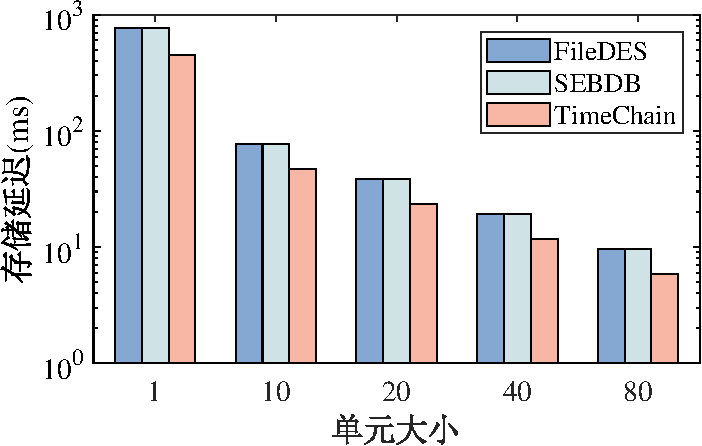
\includegraphics[width=0.6\textwidth]{figures/timechain/storage_rt_eval.pdf}
    \caption{TimeChain与基线的存储延迟对比}
    \label{fig:storage_rt_eval}
\end{figure}
本文比较了不同聚合单元大小下的存储延迟。
由于物联网设备数量众多,数据生成速度快,本文将存储延迟定义为存储10000个数据的总延迟,而不是关注单个数据的微小延迟。
如\autoref{fig:storage_rt_eval}所示,相对于FileDES和SEBDB而言,TimeChain减少了至少39\%的查询延迟。
这是因为TimeChain的高效的节点选择机制和数据验证机制。
由于TimeChain在节点选择过程中,综合考虑了节点间的距离和历史服务记录,因此选择了更近的存储节点,减少了数据传输延迟。
而且,TimeChain在传输数据的过程中,采用了基于LSH树的验证机制,减少了数据传输量,从而减少了存储延迟。

此外,随着聚合单元大小变大,存储延迟变小。
这是因为,对于相同体量的数据,当聚合单元较大时,数据在链中打包和记录的次数会减少。
然而,较大的聚合单元可能会引入较大的存储等待延迟。
因为一个聚合单元可能需要等待较长时间才可以被填满,才能被打包和记录。
具体的聚合单元大小需要根据实际数据产生速度和用户的需求来确定。
用户可以通过调整网关的聚合单元大小来控制实际的存储延迟。

\subsection{查询延迟}
\begin{figure}[t]
    \centering
    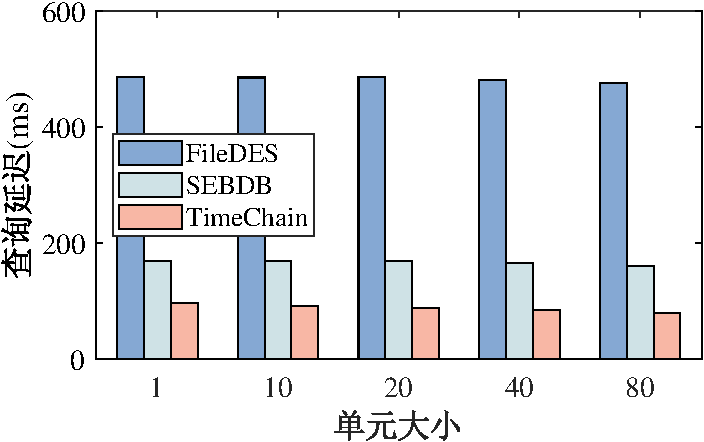
\includegraphics[width=0.6\textwidth]{figures/timechain/query_rt_eval.pdf}
    \caption{TimeChain与基线的查询延迟对比}
    \label{fig:query_rt_eval}
\end{figure}
本文比较了不同聚合单元大小的查询延迟,如\autoref{fig:query_rt_eval}所示。
查询延迟是指基于固定查询范围随机查询数据集的平均延迟。
由于不同数据集对应的数据生成速度与查询范围不同,经过综合权衡,本文选择了能耗和数据采集频率适用较广的RT-IFTTT数据集作为缺省查询工作负载。
因此,本文将缺省查询范围设置为20。

从\autoref{fig:query_rt_eval}可以看出,相比于SEBDB,TimeChain平均减少了61.9\%的查询延迟;相比于FileDES,TimeChain平均减少了84.9\%的查询延迟。
这是由于TimeChain减少了数据传输延迟,原因将在\autoref{fig:query_breakdown}中解释。

本文还发现,当聚合单元大小增加时,查询延迟会减少。
这是因为当聚合单元大小增加时,同一查询中涉及的聚合单元数量会减少,用户的查询结果将大概率集中在一个存储节点上。
然而,聚合单元越大,TimeChain相对于其他解决方案的改进将随着聚合单元的增大而减少。
这是因为当聚合单元非常大时,相当于将所有数据存储在一个聚合单元中。
在这种情况下,对于数据进行谱聚类切分不会导致性能提高,反而会导致对多种范围查询的灵活性降低。
此外,当大量数据集中在存储节点中时,存储系统的可扩展性和可靠性也会受到损害。

\subsection{查询延迟分解}
本文进一步分析了查询延迟的细分,以确定影响整体查询性能的主要因素,如\autoref{fig:query_breakdown}所示。
查询的延迟主要由4个阶段组成,检索、传输、验证和返回。
考虑到传感器通常选择更近的网关,返回阶段的延迟几乎可以忽略不计。
在验证阶段,三种方案的延迟相对接近,小于1ms,也可以被忽略。

在传输和检索阶段,本文发现延迟占据了查询延迟的主要部分。
特别是TimeChain的传输延迟明显低于FileDES和SEBDB。
这一优势归功于TimeChain的节点打包机制,该机制优化了数据的组织方式,减少了从存储节点获取数据的次数。
同时,TimeChain的节点选择机制通过选择地理位置更近的存储提供商进一步缩短了数据传输的距离,从而降低了传输延迟。

在检索阶段,FileDES由于需要遍历区块链上的所有块来检索数据,导致了较高的检索延迟。
这种机制在面对大量数据时效率较低,尤其是在数据量迅速增长的场景下。
相比之下,SEBDB和TimeChain通过使用B+树和R树索引结构,显著提高了检索效率,降低了延迟。
这两种索引结构允许系统快速定位到存储数据的位置,从而加快了检索速度。
\begin{figure}[t]
    \centering
    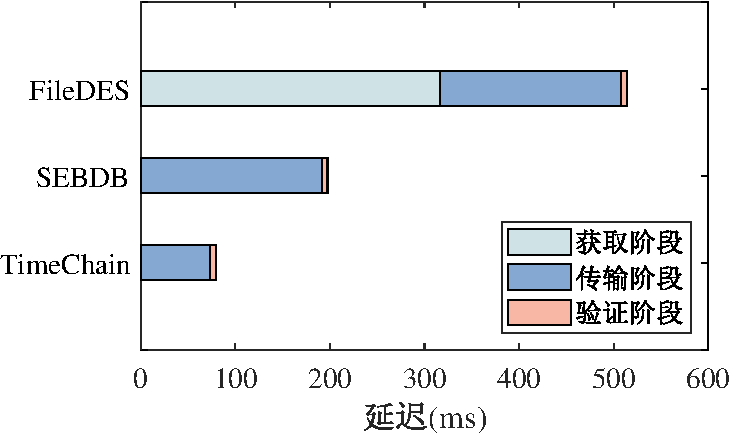
\includegraphics[width=0.6\linewidth]{figures/timechain/query_breakdown.pdf}
    \caption{查询延迟分解对比}
    \label{fig:query_breakdown}
\end{figure}

\subsection{支持的最大存储设备数量}
在本小节中,本文使用的支持设备最大数量指标,即存储系统每秒可以提供存储服务的设备数量。
本文假设网关可以同时处理来自多个物联网设备的数据存储请求,并忽略网关本身的处理延迟。
所有物联网设备同时以1Hz的频率生成数据,并要求在生成下一个数据之前必须存储这些数据。
在这样的限制下,存储系统可以并行支持的最多设备数量即为支持的最大存储设备数量。

如\autoref{fig:support_device}所示,TimeChain支持最大设备数量分别是SEBDB和FileDES的1.63倍和3.55倍。
这主要是由于TimeChain对数据传输延迟采取的优化技术,较小的数据传输延迟允许TimeChain以更快的速度存储数据。
此外,对于所有测试的方案而言,随着聚合单元大小的增加,支持的最大设备数量也随之增加。
这是因为较大的聚合单元意味着单个链上哈希可以代表更多的数据量,从而提高了单个存储单元的效率,使得系统能够支持更多的物联网设备。

特别地,当聚合单元大小达到80时,TimeChain支持的最大设备数已经达到了千级,这一结果充分展示了TimeChain在大规模物联网环境中的扩展能力和高效性。
这一性能优势不仅证明了TimeChain在处理大规模数据时的可靠性,也为未来物联网应用的发展提供了强有力的技术支持。
\begin{figure}[t]
    \centering
    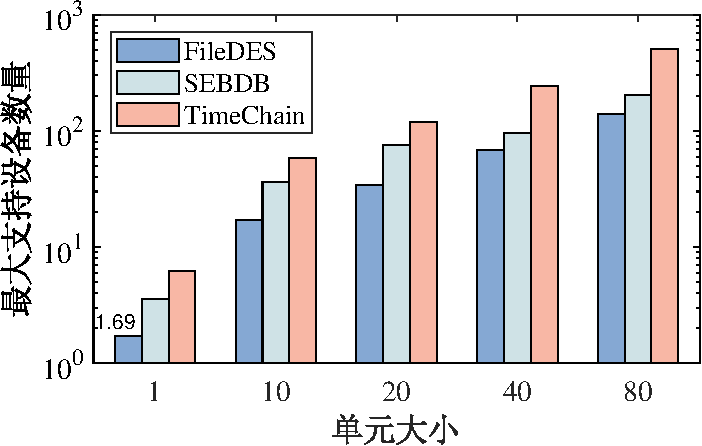
\includegraphics[width=0.6\linewidth]{figures/timechain/support_device.pdf}
    \caption{最大支持存储设备数}
    \label{fig:support_device}
\end{figure}

\section{性能影响因素评估}
\subsection{不同查询大小下的查询延迟}
本文比较了各方案在三种不同查询大小数据集(Bridge、RT和WX)的查询性能,结果如\autoref{fig:query_diff_dataset}所示。
三个数据集中工作负载的平均查询大小分别为40、20和10。
本文可以发现,这三种解决方案的查询延迟通常随着查询大小的增加而增加,即WX最小,RT次之,Bridge最大。
这是因为更大的查询大小涉及了更多的聚合单元,因此可能需要去更多的存储节点获取数据,从而增加了数据传输延迟。

本文观察到,与SEBDB和FileDES相比,当查询大小变大时,TimeChain的聚类算法带来的性能改进也会增加。
具体来说,SEBDB和FileDES在处理较大的查询时,通常需要从比TimeChain更多的节点获取数据,这导致了较高的数据传输延迟。
而TimeChain通过其先进的聚类算法,能够有效减少数据获取的次数,进而显著降低数据传输延迟,从而在面对较大查询时展现出更优的性能表现。
这一特性使得TimeChain在处理大规模查询时具有显著的优势,能够更好地满足物联网场景下对高效数据查询的需求。

\subsection{不同存储网络规模下的存储延迟}
\begin{figure}[t]
    \centering
	\begin{minipage}{0.48\linewidth}
        \centering
        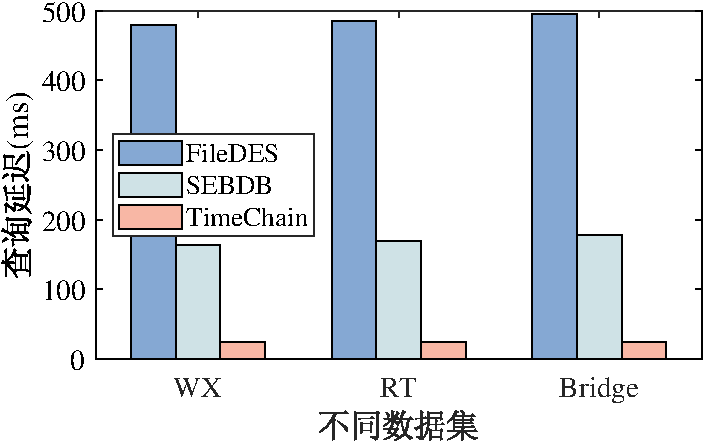
\includegraphics[width=1\textwidth]{figures/timechain/query_diff_dataset.pdf}
        \caption{不同查询大小下的查询延迟}
        \label{fig:query_diff_dataset}
	\end{minipage}
	\quad
	\begin{minipage}{0.48\linewidth}
        \centering
        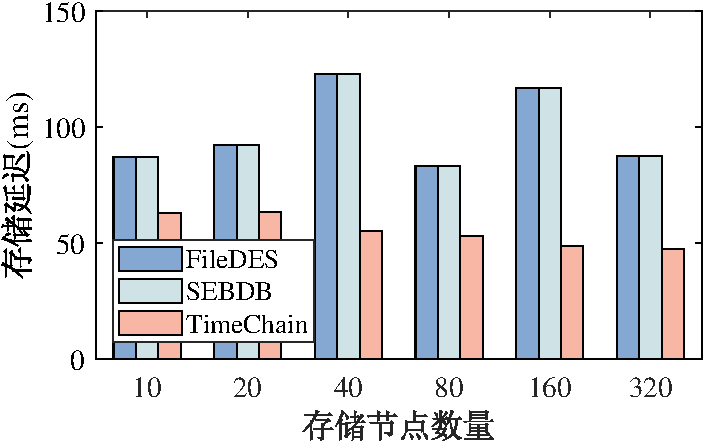
\includegraphics[width=1\textwidth]{figures/timechain/storage_diff_storage_nodes.pdf}
        \caption{不同存储网络下的存储延迟}
        \label{fig:storage_diff_storage_nodes}
    \end{minipage}
\end{figure}

本文比较了不同存储网络规模下每种解决方案的存储延迟,结果如\autoref{fig:storage_diff_storage_nodes}所示。
随着存储节点数量的增加,TimeChain的存储延迟呈现出明显的下降趋势。
具体而言,当存储节点数量增加时,TimeChain可以从更多的节点中进行选择,从而增加了选择到地理位置更接近的存储节点的机会。
这种选择机制自然降低了数据传输的时间,进而有效减少了存储延迟。

相比之下,FileDES和SEBDB在存储节点数量增加时,并没有表现出存储延迟的显著变化。
这是因为在节点选择过程中,它们根据存储节点的信誉随机选择可靠节点,而不考虑节点的具体位置信息。
这种随机性导致了这两种方案在存储延迟上缺乏可预测性。
在不同存储网络规模下,它们的性能波动较大,无法像TimeChain那样通过优化节点选择来降低延迟。
由于FileDES和SEBDB在选择存储节点时没有考虑节点的具体位置信息,它们无法充分利用增加的节点来优化存储延迟。
这就导致了即使在存储节点数量增加的情况下,这两种方案的存储延迟仍然保持在一个相对较高的水平,且波动较大。
这种较高的延迟和较大的波动在一定程度上限制了它们在大规模存储网络中的应用潜力。

\section{消融实验}
\subsection{聚类算法}
\begin{figure*}[t]
    \centering
	\begin{minipage}{1\linewidth}
        \subfigure[查询延迟]{
            \centering
            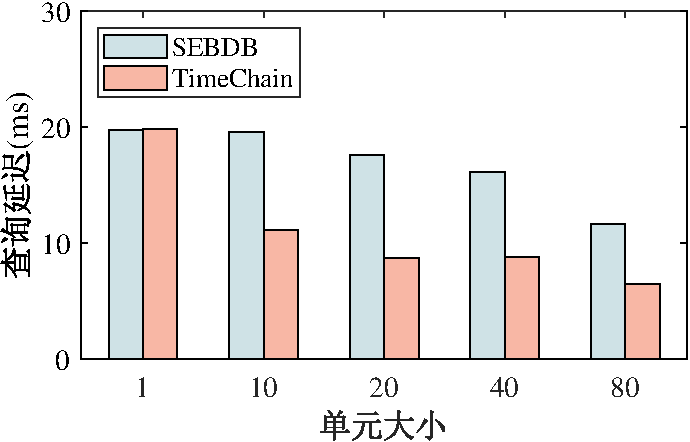
\includegraphics[width=0.48\textwidth]{figures/timechain/ratiocut_latency_eval.pdf}
        }
        \quad
        \subfigure[跨越的batch]{
            \centering
            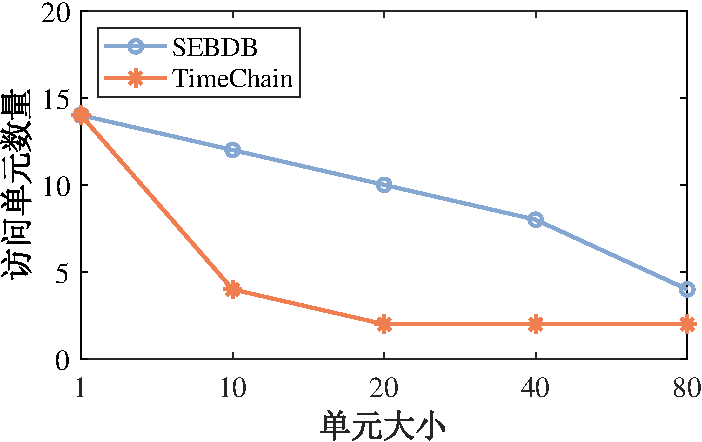
\includegraphics[width=0.48\textwidth]{figures/timechain/ratiocut_batch_eval.pdf}
        }
        \caption{聚类算法消融实验} 
        \label{fig:ratiocut_eval}
    \end{minipage}
\end{figure*}

本文比较了聚类算法的效果,并将TimeChain与SEBDB进行了比较。
如\autoref{fig:ratiocut_eval}(a)所示,与SEBDB相比,TimeChain的网络传输延迟减少了40.3\%。
这是因为SEBDB的打包节点未能充分考虑用户查询的规律性,只是将物联网数据根据到达网关的顺序进行打包。
这导致在处理数据拥有者请求的数据时,SEBDB不得不访问多个存储提供商所管理的聚合单元,增加了数据检索的复杂性和延迟。
相比之下,TimeChain采用了谱聚类算法,这种算法能够根据用户请求的特征对来自特定传感器的数据进行打包。
这种方法不仅优化了数据在存储节点中的分布,还减少了数据访问时需要跨越的聚合单元数量。
如\autoref{fig:ratiocut_eval}(b)所示,TimeChain访问的聚合单元数量比SEBDB少了59.3\%,这表明TimeChain在减少数据访问延迟和提高查询效率方面具有明显优势。

\begin{figure*}[t]
    \centering
    \begin{minipage}{1\linewidth}
        \subfigure[查询延迟]{
            \centering
            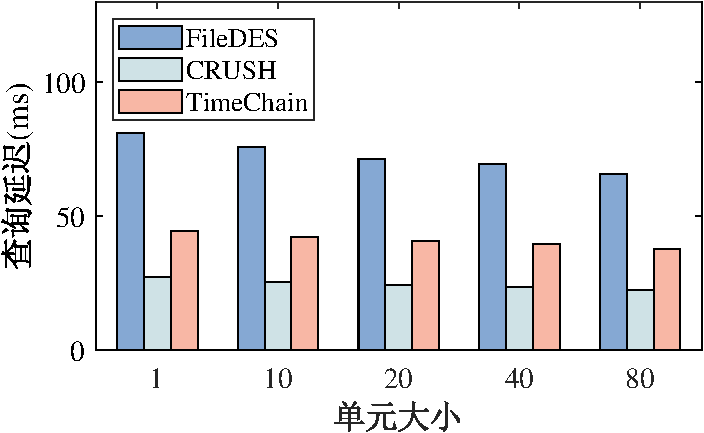
\includegraphics[width=0.48\textwidth]{figures/timechain/consensus_latency_eval.pdf}
        }
        \quad
        \subfigure[存储服务质量]{
            \centering
            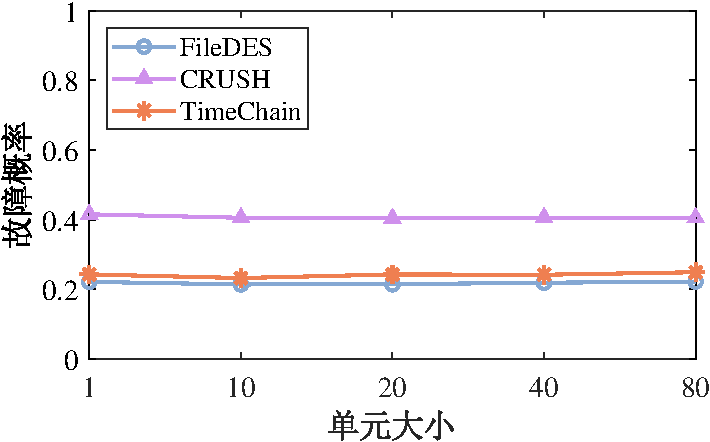
\includegraphics[width=0.48\textwidth]{figures/timechain/consensus_prob_eval.pdf}
        }
        \caption{节点选择消融实验} 
        \label{fig:consensus_eval}
    \end{minipage}
\end{figure*}

\subsection{节点选择}
本文在\autoref{fig:consensus_eval}中显示了TimeChain、FileDES~\cite{xu2024filedes}和CRUSH~\cite{weil2006ceph}在节点选择方面的性能差异。

FileDES通过基于节点信誉的筛选机制,确定了一组受信任的存储节点,并在此基础上随机选择节点进行数据存储。
这种方法的优点在于提高了数据存储的安全性,因为只有信誉良好的节点才被考虑用于存储。
然而,由于缺乏对节点地理位置的考虑,FileDES的随机选择可能导致选择了距离较远的节点,从而增加了数据传输的延迟,影响了整体性能。

CRUSH则采取了一种基于物理位置的策略,优先选择距离最近的节点进行数据存储。
这种策略在不考虑节点故障和可靠性的情况下,能够显著减少数据传输的时间。
然而,CRUSH方案的一个主要缺陷是它没有充分考虑节点的可靠性,如\autoref{fig:consensus_eval}(b)所示,这导致有41\%的节点可能无法提供有效的存储服务,这对于需要高可靠性的存储系统来说是一个严重的缺陷。

与FileDES和CRUSH相比,TimeChain在节点选择上采取了一种综合考虑节点物理距离和信誉的策略。
TimeChain不仅考虑了节点的地理位置以减少传输延迟,还考虑了节点的历史服务记录和信誉,以确保所选节点的可靠性。
这种综合考虑的方法使得TimeChain在响应时间和服务概率方面都展现出了最佳性能。
尽管TimeChain选择的节点可能不是物理距离上最近的,但通过平衡节点的距离和服务质量,TimeChain能够提供更稳定和高效的存储服务。

\subsection{LSH树}

\begin{figure*}[t]
    \centering
    \begin{minipage}{1\linewidth}
        \subfigure[查询延迟]{
            \centering
            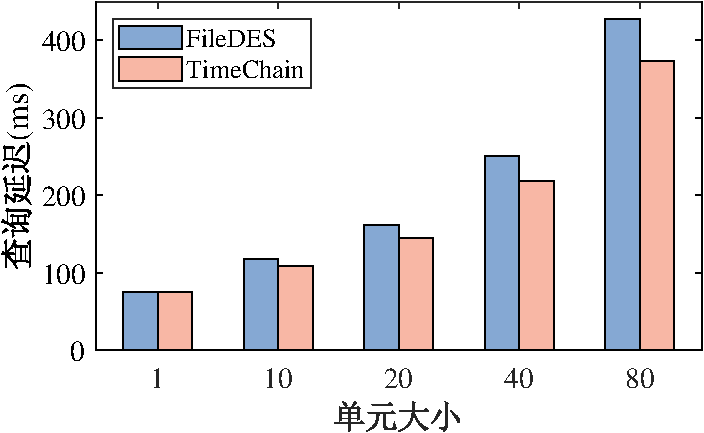
\includegraphics[width=0.48\textwidth]{figures/timechain/lsh_latency_eval.pdf}
        }
        \quad
        \subfigure[完整性证明大小]{
            \centering
            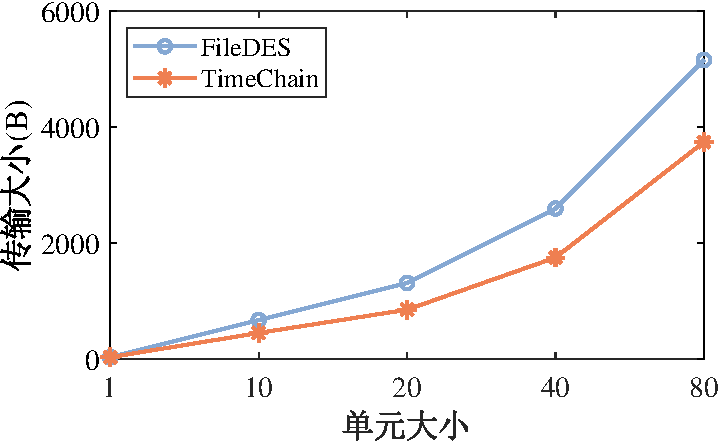
\includegraphics[width=0.48\textwidth]{figures/timechain/lsh_size_eval.pdf}
        }
        \caption{LSH树消融实验} 
        \label{fig:lsh_eval}
    \end{minipage}
\end{figure*}
本文比较了FileDES和TimeChain的网络传输延迟,如\autoref{fig:lsh_eval}(a)所示。
与FileDES相比,TimeChain的数据传输延迟减少了10.9\%。
这主要是来源于TimeChain对数据传输量的优化。
在物联网中,局域网内传感器设备的数量众多,且这些设备通常以高频率持续生成数据。
而且,TimeChain相比于FileDES的传输优化随着数据量的增加而增加。
这是因为当数据量增加时,LSH树中的相似数据量也会增加,从而减少了传输的数据量,降低了网络传输延迟。

如\autoref{fig:lsh_eval}(b)所示,由于TimeChain使用LSH作为哈希算法,通过网络传输的数据量大大减少。
这种数据量的减少不仅降低了存储和查询操作的延迟,还显著减轻了存储提供商的存储负担。
对于存储提供商而言,这意味着更低的存储成本和更高的数据处理效率。
同时,对于整个存储系统来说,减少了数据传输量还有助于提高系统的吞吐量和响应速度,尤其是在高负载或资源受限的环境中。

\section{本章小结}
本章对TimeChain系统进行了全面的实验评估,以验证其在存储性能方面的优势。
通过在模拟的全球存储网络上进行测试,本章比较了TimeChain与现有解决方案,SEBDB和FileDES,在存储延迟和查询延迟方面的表现。
实验结果表明,TimeChain在减少查询延迟和存储延迟方面具有显著优势,平均查询延迟降低了64.6\%,存储延迟降低了35.3\%。

本章还分析了不同查询负载和存储网络规模对TimeChain性能的影响,发现随着聚合单元大小的增加,TimeChain的存储和查询性能得到了进一步的提升。
此外,TimeChain在支持最大存储设备数量方面也展现出了其可扩展性,与SEBDB和FileDES相比,分别增加了1.63倍和3.55倍。

为了进一步验证TimeChain设计中关键技术点的有效性,本章进行了消融实验。
实验结果证实了自适应聚合机制、基于共识的节点选择机制和基于LSH树的验证机制在提升系统性能方面的重要作用。
特别是LSH树机制,通过减少传输的数据量,显著降低了网络传输延迟。
